%
% chapter.tex
%
% (c) 2025 Prof Dr Andreas Müller
%
\chapter{$p$-Formen und das Poincaré-Lemma
\label{chapter:pformen}}
\kopflinks{$p$-Formen und das Poincaré-Lemma}

\noindent
In Abschnitt~\ref{buch:green:section:geschlossen} wurde gezeigt, dass eine
1-Form $\alpha$ mit $d\alpha=1$ in einem einfach zusammenhängenden Gebiet
mit Hilfe des Kurvenintegrals als Differential $df=\alpha$ einer Funktion
$f$ schreiben lässt.
In Kapitel~\ref{chapter:gauss} wurde angedeutet, dass etwas Ähnliches auch
für eine 2-Form auf $\mathbb{R}^3$ gilt.
In der Vektorsprache lässt sich ein Vektorfeld, welches verschwindende
Divergenz hat, als Rotation eines Vektorfeldes schreiben.
In diesem Kapitel soll gezeigt werden, dass beides nur Spezialfälle sind.
Dazu wird die allgemeine Theorie der $p$-Formen und der äusseren Ableitung
auf einer Mannigfaltigkeit entwickelt und gezeigt, 

%
% p-Formen
%
\section{$p$-Formen
\label{buch:pformen:section:pformen}}
\kopfrechts{$p$-Formen}
Im ersten Schritt müssen die Begriffe der 2-Vektoren und der 
Differentialformen auf Vektoren und Formen beliebigen Grades
verallgemeinert werden.

%
% p-Vektoren
%
\subsection{$p$-Vektoren}
In früheren Kapiteln würden 2-Vektoren, $(n-1)$-Vektoren und $n$-Vektoren
eingeführt, sobald sie für die Erklärung der Sätze von Green,
Stokes und Gauss nötig waren.
Die Konstruktion lässt sich aber auf den Begriff eines $p$-Vektors
für beliebiges $p$ auf einer $n$-dimensionalen Mannigfaltigkeit
verallgemeinern.

\begin{definition}
Ein $p$-Vektor ist ein vollständig antisymmetrischer Tensor
$p$-ter Stufe vom Typ $(0,p)$.
\end{definition}

Aus einer Basis $X_1,\dots,X_n$ von $TM$ entsteht eine Basis des
Vektorraums der $p$-Vektoren besteht daher mit den
total antisymmetrischen Tensoren
\[
X_{i_1}\wedge \dots\wedge X_{i_p}
=
\sum_{k_1,\dots,k_p=1}^{n}
\varepsilon_{k_1\dots k_p}
X_{i_{k_1}}\otimes\dots\otimes X_{i_{k_p}}
\]
Darin ist $\varepsilon_{k_1\dots k_p}$ ist das Levi-Cività-Symbol
$p$-ter Stufe.
Der Vektorraum der $p$-Vektoren wird auch als 
$\bigwedge^p TM$ geschrieben.

%
% Antisymmetrische Multilinearformen
%
\subsection{Antisymmetrische Multilinearformen auf $TM$}
Dual zu den $p$-Vektoren sind die Linearformen auf einer $n$-dimensionalen
Mannigfaltigkeit sind die $p$-Formen.

\begin{definition}
Eine $p$-Form auf der $n$-dimensionalen Mannigfaltigkeit ist eine vollständig
antisymmetrische Multilinearform vom Grad $p$.
Die $p$-Formen $dx^{i_1}\wedge\dots\wedge dx^{i_p}$ sind dual zu den 
$p$-Vektoren $X_{i_1}\wedge\dots\wedge X_{i_p}$:
\[
\langle
dx^{i_1}\wedge\dots\wedge dx^{i_p},
X_{k_1}\wedge\dots\wedge X_{k_p}
\rangle
=
\delta^{i_1}_{k_1}
\dots
\delta^{i_p}_{k_p}.
\]
Die Menge der $p$-Formen auf einer Mannigfaltigkeit wird mit $\Omega^p(M)$
bezeichnet.
\end{definition}

Die Menge $\Omega^0(M)$ der $0$-Formen besteht nur aus beliebig oft stetig
differenzierbaren Funktionen auf der Mannigfaltigkeit, die mit
$C^\infty(M)$ bezeichnet wird.
Die $p$-Formen im Vektorraum der $p$-Formen können mit Funktionen aus
$C^\infty(M)$ multipliziert werden, eine Eigenschaft, die man einen
$C^\infty(M)$-Modul nennt.

\begin{satz}
Die $p$-Formen auf einer Mannigfaltigkeit bilden einen $C^\infty(M)$-Modul.
In einer Karte kann eine $p$-Form $\omega\in \Omega^p(M)$ als
\begin{align*}
\omega
&=
\sum_{i_1<i_2<\dots< i_p}
f_{i_1 i_2\dots i_p}(x)
\, dx^{i_1}\wedge dx^{i_2}\wedge\dots\wedge dx^{i_p}
\\
&=
\frac{1}{p!}
\sum_{i_1,i_2,\dots,i_p}
f_{i_1 2_2\dots i_p}(x)
\, dx^{i_1}\wedge dx^{i_2}\wedge\dots\wedge dx^{i_p}
\end{align*}
geschrieben werden, wobei $f_{i_1 i_2\dots i_p}$  antisymmetrisch ist in jedem
Indexpaar.
\end{satz}

%
% Das \wedge-Produkt von $p$-Formen
%
\subsection{Das $\wedge$-Produkt}
Das Wedge-Produkt von Differentialformen ist eine bilineare Abbildung
\[
\Omega^p(M)\times \Omega^q(M) \to \Omega^{p+q}(M)
:
(\alpha,\beta) \mapsto \alpha\wedge\beta.
\]
Dies bedeutet, dass es ausreicht, das Wedge-Produkt auf einer Basis
zu definieren.

Seien jetzt also
\begin{align*}
\alpha &= dx^{i_1}\wedge\dots\wedge dx^{i_p} \\
\beta  &= dx^{j_{p+1}}\wedge\dots\wedge dx^{j_{p+q}}
\end{align*}
zwei Basis-$p$- bzw.~-$q$-Formen.
Es muss das Produkt
\begin{equation}
dx^{i_1}\wedge\dots\wedge dx^{i_p}
\wedge
dx^{i_{p+1}}\wedge\dots\wedge dx^{i_{p+q}}
\label{buch:pformen:pformen:eqn:basisprodukt}
\end{equation}
durch Basis-$(p+q)$-Formen ausgedrückt werden.
Falls $(i_1,\dots,i_p)$ und $(i_{p+1},\dots,i_{p+q})$ einen Index gemeinsam
haben, dann verschwindet das Produkt.
Das Wedge-Produkt~\eqref{buch:pformen:pformen:eqn:basisprodukt}
ist also nur dann von $0$ verschieden, wenn alle Indizes in
$(i_1,\dots,i_p,i_{p+1},\dots,i_{p+q})$ verschieden sind.
Das Produkt~\eqref{buch:pformen:pformen:eqn:basisprodukt} ist aber
normalerweise keine Basis-$(p+q)$-Form, da in den Basisformen die
Indizes aufsteigend sind.
Die 1-Formen in \eqref{buch:pformen:pformen:eqn:basisprodukt} müssen
also so vertauscht werden, dass sich eine aufsteigende Reihenfolge
$(k_1,\dots,k_{p+q})$
der Indizes ergibt.
Bei jeder Vertauschung ändert das Vorzeichen.
Das Produkt \eqref{buch:pformen:pformen:eqn:basisprodukt} unterscheidet
sich also nur durch das Vorzeichen von 
\(
dx^{k_1}\wedge\dots\wedge dx^{k_{p+q}}
\).

Zur Bestimmung des Vorzeichens des Produktes $\alpha\wedge\beta$ 
sei $\sigma\in S_{p+q}$ die Permutation\footnote{Die Theorie der
Permutationen, der Gruppen $S_n$ und des Vorzeichens einer Permutation
wird ausführlich erklärt in \cite[Abschnitt~4.3.4]{buch:linalg}.}
der Zahlen $1,\dots,p+q$,
die $(i_1,\dots,i_p,i_{p+1},\dots,i_{p+q})$ in die geordnete
Reihenfolge
\[
(i_{\sigma(1)},\dots,i_{\sigma(p)},i_{\sigma(p+1)},\dots,i_{\sigma(p+q)})
=
(k_1,\dots,k_{p+q})
\]
überführt.
Die Anzahl $t(\sigma)$ der Vertauschungen, mit denen sich die
Permutation $\sigma$ schreiben lässt, ist nicht eindeutig bestimmt,
aber sie ist entweder gerade oder ungerade.
Das gesuchte Vorzeichen ist daher das sogenannte Signum
\[
\operatorname{sgn}(\sigma) = (-1)^{t(\sigma)}
\]
oder Vorzeichen der Permutation.

%
% Die Summenformel
%
\subsubsection{Die Summenformel}
Bei der konkreten Berechnung eines Wedge-Produktes ist es jeweils
einfach, die nötigen Vertauschungen vorzunehmen und damit das
richtige Vorzeichen zu finden.
Für die algebraische Rechnung ist dies jedoch etwas komplizierter,
da die Algebra keine gute Notation für die richtige Reihenfolge der
Indizes anbietet.

Um eine einfachere Formel zu finden, schreiben wir erst die Basis
auf eine neue Art.
Statt als Basisvektoren die Produkte von 1-Formen in einer vorgegebenen
Reihenfolge zu nehmen, lassen wir alle Reihenfolgen der Indizes zu.
Die so entstehenden Produkte unterscheiden sich nur durch ein
Vorzeichen.
Jedes der Produkte
\[
dx^{i_1}\wedge\dots\wedge dx^{i_p}
=
\operatorname{sgn}(\sigma)
\,
dx^{i_{\sigma(1)}} \wedge\dots\wedge dx^{i_{\sigma(p)}}
\]
für eine Permutation $\sigma\in S_p$ ist also gleichermassen geeignet
als Basisvektor.
Es gibt $p!$ solche Permutationen.
Damit wir die verschiedenen Basisvektoren gleichberechtigt verwenden
können, nehmen wir deren Mittelwert
\[
dx^{i_1}\wedge\dots\wedge dx^{i_p}
=
\frac{1}{p!}
\sum_{\sigma\in S_p} dx^{i_{\sigma(1)}} \wedge\dots\wedge dx^{i_{\sigma(p)}}
\]
Diese Summe ändert nicht, wenn die Indizes $i_1,\dots,i_p$ mit einer
geraden Permutation permutiert werden.

Eine beliebige $p$-Form ist in der Basis der
$dx^{i_1}\wedge\dots\wedge dx^{i_p}$  mit $i_1<\dots<i_p$
durch die Koeffizienten $f_{i_1\dots i_p}$ gegeben.
Die Forderung der aufsteigend sortierten Indizes in
\[
\omega
=
\sum_{i_1<\dots<i_p}
f_{i_1\dots i_p}\,
dx^{i_1}\wedge\dots\wedge dx^{i_p}
\]
ist etwas schwerfällig.
Die Beschreibung wird einfacher, wenn man verlangt, dass die
Koeffizienten vollständig antisymmetrisch sind, also
\[
f_{i_1\dots i_p}
=
\operatorname{sgn}\,
f_{i_{\sigma(1)}\dots i_{\sigma(p)}}
\]
für jede Permutation $\sigma\in S_p$.
Damit fällt jetzt die Foderung nach aufsteigenden Indizes weg und man
kann
\begin{equation}
\omega
=
\frac{1}{p!}
\sum_{i_1,\dots,i_p=1}^n
f_{i_1\dots i_p}
\,
dx^{i_1}\wedge\dots\wedge dx^{i_p}
\label{buch:pformen:pformen:eqn:summenformel}
\end{equation}
schreiben.

%
% Kommutativität
%
\subsubsection{Kommutativität}
Das Wedge-Produkt ist nicht kommutativ.
Für 1-Formen gilt $dx^i\wedge dx^k=-dx^k\wedge dx^i$.
Es ist aber auch nicht antikommutativ, denn 
\[
(dx^2\wedge dx^3)\wedge dx^1
=
-dx^2\wedge dx^1\wedge dx^3
=
dx^1\wedge dx^2\wedge dx^3,
\]
in diesem Fall ändert das Vorzeichen bei der Vertauschung der
Faktoren $dx^1$ und $dx^2\wedge dx^3$ nicht.
Der Grund ist, dass {\em zwei} Vertauschungen nötig sind, um
die Faktoren in die Standardreihenfolge zu bringen.
Wir beweisen die folgende Kommutationsformel.

\begin{satz}
Für eine $p$-Form $\alpha\in\Omega^p(M)$ und eine $q$-Form
$\beta\in\Omega^q(M)$ gilt
\begin{equation}
\alpha\wedge\beta
=
(-1)^{pq}\,\beta\wedge\alpha.
\label{buch:pformen:pformen:eqn:kommutativ}
\end{equation}
\end{satz}

\begin{proof}
Wir müssen zeigen, dass die
Formel~\eqref{buch:pformen:pformen:eqn:kommutativ}
Für die Basisdifferentialformen gilt.
Wir verwenden die Farben {\color{darkred}rot} und {\color{blue}blau},
um die Vertauschungen der 1-Form-Faktoren deutlich zu machen.
Wir schreiben also
\begin{align*}
{\color{darkred}\alpha}
&=
{\color{darkred}dx^{i_1}}
\wedge \dots \wedge
{\color{darkred}dx^{i_p}}
\\
\text{und}\qquad
{\color{blue}\beta}
&=
{\color{blue}dx^{k_1}}
\wedge \dots \wedge
{\color{blue}dx^{k_p}}
\end{align*}
und berechnen die Produkte $\alpha\wedge\beta$ und $\beta\wedge\alpha$.
Um das Produkt $\beta\wedge\alpha$ in die Reihenfolge der 1-Form-Faktoren
von $\alpha\wedge\beta$ zu bringen, sind jeweils Vertauschungen mit
Nachbarfaktoren notwendig:
\begin{align*}
{\color{darkred}\alpha}\wedge{\color{blue}\beta}
&=
{\color{darkred}dx^{i_1}}
\wedge\dots\wedge
{\color{darkred}dx^{i_p}}
\wedge
{\color{blue}dx^{k_1}}
\wedge\dots\wedge
{\color{blue}dx^{k_q}}
\\
&=
{\color{darkred}dx^{i_1}}
\wedge\dots\wedge
{\color{blue}dx^{k_1}}
\wedge
{\color{darkred}dx^{i_p}}
\wedge
{\color{blue}dx^{k_2}}
\wedge\dots\wedge
{\color{blue}dx^{k_q}}
\\
&=
(-1)^p
\,
{\color{blue}dx^{k_1}}
\wedge
{\color{darkred}dx^{i_1}}
\wedge\dots\wedge
{\color{darkred}dx^{i_p}}
\wedge
{\color{blue}dx^{k_2}}
\wedge\dots\wedge
{\color{blue} dx^{k_q}}
\\
&=
(-1)^2q
\,
{\color{blue}dx^{k_1}}
\wedge
{\color{blue}dx^{k_2}}
\wedge
{\color{darkred}dx^{i_1}}
\wedge\dots\wedge
{\color{darkred}dx^{i_p}}
\wedge
{\color{blue}dx^{k_3}}
\wedge\dots\wedge
{\color{blue} dx^{k_q}}
\\
&=
(-1)^{pq}
\,
{\color{blue}dx^{k_1}}
\wedge\dots\wedge
{\color{blue}dx^{k_q}}
\wedge
{\color{darkred}dx^{i_1}}
\wedge\dots\wedge
{\color{darkred}dx^{i_p}}
\\
&=
(-1)^{pq}
\,
{\color{blue}\beta}\wedge{\color{darkred}\alpha}.
\end{align*}
Damit ist die Formel bewiesen.
\end{proof}

%
% Die graduierte Algebra der p-Formen
%
\subsection{Die graduierte Algebra der $p$-Formen}
Die Räume $\Omega^p(M)$ haben für verschiedene $0$ keine gemeinsamen 
nichttrivialen Formen.
Die Nullform, die auf jedem beliebigen $p$-Vektor verschwindet, kann man
aber durchaus als ein gemeinsames Element betrachten.
Rein formal kann man daher auch Linearkombinationen von $p$-Formen für
verschiedenes $p$ bilden.
So entsteht die Menge
\[
\Omega^*(M)
=
\bigoplus_{p=0}^n \Omega^p (M)
\]
der Differentialformen auf der Mannigfaltigkeit.
$\Omega^*(M)$ ist ein reeller Vektorraum: Differentialformen können mit
Zahlen multipliziert und addiert werden.

Die $0$-Formen sind die Funktionen in $C^\infty(M)$ und können mit
glatten Funktionen in $\Omega^0(M)=C^\infty(M)$ multipliziert werden.
Die glatten Funktionen bilden keinen Körper, da man durch Funktionen mit
Nullstellen nicht dividieren kann.
Die glatten Funktionen bilden aber einen sogenannten Ring. 
\index{Ring}%
Es sind alle Rechenregeln definiert, die auch in einem Körper gelten,
ausser die Existenz eines multiplikativen Inversen.

Die Differentialformen können mit Funktionen in $C^\infty(M)$
multipliziert werden.
Dadurch wird $\Omega^*(M)$ zu einem sogenannten {\em Modul} über
dem Ring $C^\infty(M)$.
Wenn $f\in C^\infty(M)$ eine glatte Funktion und $\omega\in\Omega^p(M)$
eine $p$-Form ist, dann ist $f\omega\in\Omega^p(M)$ ebenfalls eine
$p$-Form.
Die Multiplikation mit einer glatten Funktion ändert den Grad einer
$p$-Form nicht.
Jeder einzelne Summand $\Omega^p(M)\subset\Omega^*(M)$ ist also für
sich genommen ebenfalls ein $C^\infty(M)$-Modul.
Man nennt $\Omega^*(M)$ daher einen {\em graduierten} $C^\infty(M)$-Modul.
\index{graduiert}%
\index{Modul, graduiert}%

Das Wedge-Produkt der Differentialformen verknüpft eine $p$-Form
$\alpha\in\Omega^p(M)$ mit einer $q$-Form $\beta\in\Omega^q(M)$
zu einer $p+q$-Form $\alpha\wedge\beta\in\Omega^{p+q}(M)$.
Die Menge $\Omega^*(M)$ hat also nicht nur die Struktur eines
Moduls über dem Ring $C^\infty(M)$ sondern auch die Struktur
einer Algebra über dem Ring $C^\infty(M)$.
Das Produkt respektiert aber auch die Graduierung von $\Omega^*(M)$,
daher heisst $\Omega^*(M)$ auch eine graduierte $C^\infty(M)$-Algebra.


%
% Die äussere Ableitung
%
\section{Die äussere Ableitung
\label{buch:pformen:section:aeussereableitung}}
\kopfrechts{Die äussere Ableitung}
Für 1-Formen, 2-Formen und $n-1$-Formen wurde die äussere
Ableitung bereits definiert.
Auf Basisdifferentialformen ist die äussere Ableitung
durch die ausreichend verschiedenen Formeln
\begin{align*}
d(
f\,dx^i
)
&=
\frac{\partial f}{\partial x^k}\, dx^k\wedge dx^i
\\
d(g\,dx^i\wedge dx^k)
&=
\sum_{l=1}^n
\frac{\partial g}{\partial x^l}\, dx^l\wedge dx^i\wedge dx^k
\\
d(h\,
dx^1\wedge\dots\wedge \widehat{dx^i}\wedge\dots\wedge dx^n
)
&=
\frac{\partial h}{\partial x^i}
\,
dx^i\wedge
(dx^1\wedge\dots\wedge \widehat{dx^i}\wedge\dots\wedge dx^n)
\\
&=
(-1)^{n-1}
\frac{\partial h}{\partial x^i}
\,
dx^1\wedge\dots\wedge dx^n.
\end{align*}
gegeben.
Für die weitere Entwicklung brauchen wir eine Definition, die in allen
Fällen anwendbar ist.

%
% Definition der äusseren Ableitung
%
\subsection{Definition der äusseren Ableitung}
Die äussere Ableitung ist linear, es reicht daher, sie auf
Basisdifferentialformen zu definieren.

\begin{definition}[Äussere Ableitung]
\label{buch:pformen:def:aeussereableitung}
Die äussere Ableitung der Basis-$p$-Form 
$\alpha=f(x)\, dx^{i_1}\wedge\dots\wedge dx^{i_p}$
ist
\[
d\alpha
=
\sum_{k=1}^n
\frac{\partial f}{\partial x^k}
\,dx^k\wedge
dx^{i_1}\wedge\dots\wedge dx^{i_p}.
\]
\end{definition}

Für eine beliebige $p$-Form
\[
\omega
=
\sum_{i_1<\dots <i_p}
f_{i_1\dots i_p}\, dx^{i_1}\wedge\dots\wedge dx^{i_p}
\]
kann die äussere Ableitung daher als
\[
d\omega
=
\sum_{k=1}^n
\sum_{i_1<\dots <i_p}
\frac{\partial f_{i_1\dots i_p}}{\partial x^k}
\,dx^k
\wedge
dx^{i_1}
\wedge
\dots
\wedge
dx^{i_p}
\]
geschrieben werden.
Verwendet man vollständig antisymmetrische Koeffizienten wie in
\eqref{buch:pformen:pformen:eqn:summenformel}, bekommt die
äussere Ableitung die Form
\[
d\omega
=
\frac{1}{p!}
\sum_{i_1,\dots,i_p=1}^n
\frac{\partial f_{i_1\dots i_p}}{\partial x^k}
\,
dx^k\wedge dx^{i_1}\wedge\dots\wedge dx^{i_p}.
\]

%
% Äussere Ableitung und Wedge-Produkt
%
\subsection{Äussere Ableitung und Wedge-Produkt}
Wir berechnen die äussere Ableitung des Wedge-Produkts zweier
Differentialformen.
Seien also $\alpha\in\Omega^p(M)$ und $\beta\in\Omega^q(M)$
Differentialformen auf der Mannigfaltigkeit.
Um die äussere Ableitung des Produktes $\alpha\wedge\beta$ zu
berechnen, gehen wir von einfachen Monomen
\[
\alpha
=
f\,dx^{i_1}\wedge\dots\wedge dx^{i_p}
\qquad\text{und}\qquad
\beta
=
g\,dx^{i_{p+1}}\wedge\dots\wedge dx^{i_{p+q}}
\]
aus.
Das Produkt ist
\[
\alpha\wedge\beta
=
f(x)\,g(x)\,
dx^{i_1}\wedge\dots\wedge dx^{i_p}
\wedge
dx^{i_{p+1}}\wedge\dots\wedge d^{i_{p+q}}.
\]
Die äussere Ableitung ist
\begin{align*}
d(\alpha\wedge\beta)
&=
\sum_{k=1}^n
\frac{\partial(f\cdot g)}{\partial x^k}
dx^k
\wedge
dx^{i_1}\wedge\dots\wedge dx^{i_p}
\wedge
dx^{i_{p+1}}\wedge\dots\wedge d^{i_{p+q}}
\\
&=
\sum_{k=1}^n
\biggl(
\frac{\partial f}{\partial x^k}(x)
g(x)
+
f(x)
\frac{\partial g}{\partial x^k}(x)
\biggr)\,
dx^k
\wedge
dx^{i_1}\wedge\dots\wedge dx^{i_p}
\wedge
dx^{i_{p+1}}\wedge\dots\wedge d^{i_{p+q}}
\\
&=
\sum_{k=1}^n
\frac{\partial f}{\partial x^k}(x)\,
dx^k
\wedge
dx^{i_1}\wedge\dots\wedge dx^{i_p}
\wedge
g(x)\,
dx^{i_{p+1}}\wedge\dots\wedge d^{i_{p+q}}
\\
&\qquad +
\sum_{k=1}^n
f(x)\,
dx^k
\wedge
dx^{i_1}\wedge\dots\wedge dx^{i_p}
\wedge
\frac{\partial g}{\partial x^k}(x)\,
dx^{i_{p+1}}\wedge\dots\wedge d^{i_{p+q}}.
\intertext{Um den Faktor $dx^k$ im zweiten Summanden neben
die partielle Ableitung von $g$ zu bringen, sind $p$ Vertauschungen
nötig, die Ableitung wird dann}
&=
\biggl(
\sum_{k=1}^n
\frac{\partial f}{\partial x^k}(x)\,
dx^k
\wedge
dx^{i_1}\wedge\dots\wedge dx^{i_p}
\biggr)
\wedge
g(x)\,
dx^{i_{p+1}}\wedge\dots\wedge d^{i_{p+q}}
\\
&\qquad +
f(x)\,
dx^{i_1}\wedge\dots\wedge dx^{i_p}
\wedge
(-1)^p
\sum_{k=1}^n
\frac{\partial g}{\partial x^k}(x)\,
dx^k
\wedge
dx^{i_{p+1}}\wedge\dots\wedge d^{i_{p+q}}
\\
&=
d\alpha \wedge \beta
+
(-1)^p
\alpha\wedge d\beta.
\end{align*}
Abgesehen vom zusätzlichen Vorzeichen im zweiten Term ist dies
die Produktregel.

\begin{definition}
Eine {\em Antiderivation} $d$ einer graduierten Algebra $A$ ist eine
\index{Antiderivation}%
lineare Abbildung mit
\begin{equation}
d(\alpha\cdot\beta)
=
(d\alpha)\cdot\beta
+
(-1)^p \alpha\cdot(d\beta)
\label{buch:pformen:pformen:eqn:antiderivation}
\end{equation}
für $\alpha\in A^p$ und $\beta\in A^q$.
\end{definition}

Die äussere Ableitung ist also eine Antiderivation in der graduierten
Algebra der Differentialformen auf einer Mannigfaltigkeit.
Für eine Funktion $f\in\Omega^0(M)$, $p=0$, und $\beta\in\Omega^q(M)$ 
wird aus
\eqref{buch:pformen:pformen:eqn:antiderivation}
die bekannte Produktregel
\[
d(f\beta)
=
(df)\wedge \beta
+
f\wedge d\beta.
\]

%
% Geschlossene und exakte Formen
%
\subsection{Geschlossene und exakte Formen}
Als Anwendung des Satzes von Green wurde gezeigt, dass Wegintegrale
einer 1-Form $\alpha$, deren äussere Ableitung $d\alpha$ verschwindet,
vom Weg unabhängig sind.
Es gibt dann eine Funktion $f$, deren Differential $df=\alpha$ ist.
Die Idee kann auch auf $p$-Formen ausgedehnt werden.

\begin{definition}
Eine $p$-Form $\omega$ heisst {\em geschlossen}, wenn $d\omega=0$ ist.
\index{geschlossene $p$-Form}%
Eine $p$-Form heisst {\em exakt}, wenn es eine $p-1$-Form $\alpha$ gibt,
sodass $\omega = d\alpha$.
\index{exakte $p$-Form}%
\end{definition}


%
% Die zweite äussere Ableitung
%
\subsubsection{Die zweite äussere Ableitung}
Ist $\alpha\in\Omega^p(M)$ eine $p$-Form, dann ist $d\alpha\in\Omega^{p+1}(M)$
eine $p+1$-Form.
Sie kann natürlich noch einmal mit der äusseren Ableitung differenziert
werden.

\begin{satz}
\label{buch:section:pformen:satz:zweiteableitung}
Für eine $p$-Form $\alpha\in\Omega^{p}(M)$ gilt $dd\alpha=0$.
\end{satz}

\begin{proof}
Wegen der Linearität der äusseren Ableitung genügt es, die Identität für 
eine $p$-Form der Form
\[
\alpha
=
f(x^1,\dots,x^n)\, dx^{i_1}\wedge\dots\wedge dx^{i_p}
\]
nachzurechnen.
Ausserdem dürfen wir annehmen, dass $i_1<\dots<i_p$ ist.

Die äussere Ableitung von $\alpha$ ist nach
Definition~\ref{buch:pformen:def:aeussereableitung}
\[
d\alpha
=
\sum_{k=1}^n
\frac{\partial f}{\partial x^k}
\,
dx^k\wedge
dx^{i_1}\wedge\dots\wedge dx^{i_p}.
\]
Die $p+1$-Form muss jetzt ein weiteres Mal abgeleitet werden.
Wir schreiben den neuen Index für die Koordinate, nach der abgeleitet werden
soll, mit $l$ und erhalten
\begin{align}
dd\alpha
&=
\sum_{l=1}^n 
\sum_{k=1}^n
\frac{\partial f}{\partial x^l\,\partial x^k}
\,
dx^l\wedge
dx^k\wedge
dx^{i_1}\wedge\dots\wedge dx^{i_p}.
\\
&=
\sum_{l,k=1}^n
\frac{\partial f}{\partial x^l\,\partial x^k}
\,
dx^l\wedge
dx^k\wedge
dx^{i_1}\wedge\dots\wedge dx^{i_p}.
\label{buch:pformen:ddbeweis:summe}
\intertext{Natürlich verschwinden alle Terme, in denen $l$ oder $k$ mit einem
der Indizes $i_1,\dots,i_p$ übereinstimmt.
Ebenso verschwinden die Terme mit $l=k$.
Es gibt keine Einschränkung, welcher der beiden Indizes $l$ und $k$
in~\eqref{buch:pformen:ddbeweis:summe}
grösser ist, jeder kann grösser sein.
Unterscheiden wir die beiden Fälle, erhalten wir
}
&=
\sum_{l<k}
\frac{\partial f}{\partial x^l\,\partial x^k}
\,
dx^l\wedge
dx^k\wedge
dx^{i_1}\wedge\dots\wedge dx^{i_p}.
\notag
\\
&\qquad
+
\sum_{l>k}
\frac{\partial f}{\partial x^l\,\partial x^k}
\,
dx^l\wedge
dx^k\wedge
dx^{i_1}\wedge\dots\wedge dx^{i_p}.
\notag
\intertext{Wir können die beiden Summen in eine einzige vereinen,
indem wir in der zweiten Systeme die Namen der Indizes austauschen:}
&=
\sum_{l<k}
\frac{\partial f}{\partial x^l\,\partial x^k}
\,
dx^l\wedge
dx^k\wedge
dx^{i_1}\wedge\dots\wedge dx^{i_p}.
\notag
\\
&\qquad
+
\sum_{k>l}
\frac{\partial f}{\partial x^k\,\partial x^l}
\,
dx^k\wedge
dx^l\wedge
dx^{i_1}\wedge\dots\wedge dx^{i_p}.
\notag
\intertext{Beide Summen erstrecken sich über die Paare von Indizes mit
$l<k$, wir können sie daher als eine Summe}
&=
\sum_{l<k}
\biggl(
\frac{\partial f}{\partial x^l\,\partial x^k}
dx^l\wedge dx^k
+
\frac{\partial f}{\partial x^k\,\partial x^l}
\,
dx^k\wedge
dx^l
\biggr)
\wedge
dx^{i_1}\wedge\dots\wedge dx^{i_p}.
\notag
\intertext{schreiben.
Damit die 2-Formen in der Klammer aus der Klammer gezogen werden können,
müssen wir die Faktoren im zweiten Term in der Klammer vertauschen,
wobei das Vorzeichen wechselt.
Die Summe vereinfacht sich dann zu
}
&=
\sum_{l<k}
\biggl(
\frac{\partial f}{\partial x^l\,\partial x^k}
-
\frac{\partial f}{\partial x^k\,\partial x^l}
\biggr)
\,
dx^l\wedge dx^k
\wedge
dx^{i_1}\wedge\dots\wedge dx^{i_p}.
\notag
\end{align}
Nach dem Satz von Schwarz dürfen die partiellen Ableitungen
von $f$ nach $x^k$ und $x^l$ vertauscht werden.
Die beiden Terme in der Klammer stimmen daher überein, die Klammer
verschwindet.
Daraus folgt auch, das $dd\alpha=0$ ist.
\end{proof}

%
% Äussere Ableitungen sind geschlossen und exakt
%
\subsubsection{Äussere Ableitungen sind geschlossen und exakt}
Aus dem Satz~\ref{buch:section:pformen:satz:zweiteableitung} folgt,
dass die äussere Ableitung einer beliebigen $p$-Form eine geschlossene
Form ist.
Eine äussere Ableitung einer $p$-Form ist von der Form $\omega=d\alpha$,
sie ist also nach Definition auch exakt.

Etwas schwieriger ist die Frage, ob eine geschlossene $p+1$-Form $\omega$
exakt ist.
Dazu muss eine $p$-Form $\alpha$ mit $\omega=d\alpha$ gefunden werden.
Es ist nicht offensichtlich, wie dies möglich sein soll.
Nach den Erkenntnissen von Abschnitt~\ref{buch:green:section:geschlossen}
ist eine geschlossene 1-Form auf einem zusammenhängenden Gebiet exakt.
In Abschnitt~\ref{buch:pformen:geschlossen:subsection:exakt}
wird das Poincaré-Lemma~\ref{buch:pformen:geschlossen:satz:poincare-lemma}
bewiesen, welches zeigt, dass auf einem sternförmigen Gebiet eine
geschlossene $p$-Form exakt ist.

%
% Abbildung von p-Formen
%
\section{Abbildung von $p$-Formen
\label{buch:pformen:section:abbildung}}
\kopfrechts{Abbildung von $p$-Formen}%
Beim Studium des Satzes von Stokes hat sich gezeigt, dass eine
Einbettung einer 2-dimensionalen Mannigfaltigkeit $N$ in eine beliebige
$n$-dimensionale Mannigfaltigkeit $M$ Tangentialvektoren von $N$ in
Tangentialvektoren von $M$ abgebildet werden, dass aber auch Linearformen
auf $M$ auf Linearformen in auf $N$ zurückgezogen werden können.
In diesem Abschnitt soll gezeigt werden, dass die Dimension 2
kein Spezialfall ist, sondern dass diese Konstruktion immer möglich ist.

%
% Abbildungen zwischen Mannigfaltigkeiten
%
\subsection{Abbildungen zwischen Mannigfaltigkeiten}
In diesem Abschnitt sind $N$ und $M$ Mannigfaltigkeiten der Dimension
$n$ bzw.~$m$ und $f\colon N\to M$ ist eine beliebig oft stetig
differenzierbare Abbildung von $N$ nach $M$.
Eine Funktion $h\colon M\to\mathbb{R}$ auf der Mannigfaltigkeit gibt
unmittelbar Anlass zu einer Funktion $f^*h\colon N\to\mathbb{R}$,
die sich durch Zusammensetzung $f^*h=h\circ f$ ergibt.

%
% Abbildung von Vektoren
%
\subsubsection{Abbildung von Vektoren}
Die Ableitung von $f$ definiert eine lineare Abbildung $Tf$ der
Tangentialvektoren $T_pN$ von $N$ in einem Punkt $p$ in die
Tangentialvektoren $T_{f(p)}M$ von $M$ im Punkt $f(p)$.
Wir betrachten eine Karte $(V,\varphi)$ von $N$ in der Umgebung des Punktes
$p$ und eine Karte $(U,\psi)$ von $M$ in der Umgebung von $f(p)$.
Der Einfachheit halber nehmen wir an, dass $f(V)\subset U$ ist, was wird
nötigenfalls durch Verkleinern von $V$ immer erreichen können.
In den Karten $(V,\varphi)$ und $(U,\psi)$ wird die Abbildung
$f$ zu einer glatten Abbildung
\[
\tilde{f}
=
\psi\circ f\circ\varphi^{-1}
\colon
\varphi(V)\to\psi(U)
:
q\mapsto \psi\circ f\circ \varphi^{-1}(q)
\]
zwischen offenen Mengen von $\mathbb{R}^n$ bzw.~$\mathbb{R}^m$.
Ist $\gamma\colon I\to \varphi(V)$ eine Kurve durch den Punkt $\varphi(p)$
in $\varphi(V)$, dann ist die Zusammensetzung $g\circ \gamma$
eine Kurve durch den Punkt $\psi(f(p))$ in $\psi(U)$.
In Koordinaten wird die Abbildung durch die Matrix der partiellen
Ableitungen
\[
Dg
=
\renewcommand\arraystretch{2.0}
\begin{pmatrix}
 \displaystyle\frac{\partial g^1}{\partial x^1}
&\displaystyle\frac{\partial g^1}{\partial x^2}
&\dots&
 \displaystyle\frac{\partial g^1}{\partial x^n}
\\
 \displaystyle\frac{\partial g^2}{\partial x^1}
&\displaystyle\frac{\partial g^2}{\partial x^2}
&\dots&
 \displaystyle\frac{\partial g^2}{\partial x^n}
\\[-1pt]
\vdots&\vdots&\ddots&\vdots
\\[-3pt]
 \displaystyle\frac{\partial g^m}{\partial x^1}
&\displaystyle\frac{\partial g^m}{\partial x^2}
&\dots&
 \displaystyle\frac{\partial g^m}{\partial x^n}
\end{pmatrix}
\]
gegegben.
Die Ableitung $D\tilde{f}$ bildet damit Tangentialvektoren von $N$
auf Tangentialvektoren von $M$ ab.

%
% Abbildung von p-Vektoren
%
\subsubsection{Abbildung von $p$-Vektoren}
Die Abbildung $Tf$ bildet kann auch auf Tensoren beliebiger Stufe und
insbesondere auf $p$-Vektoren ausgedehnt werden.
Die Abbildung $Tf^{\otimes p}$ bildet einen kontravarianten Tensor
$p$-ter Stufe gemäss
\[
\renewcommand{\arraycolsep}{1.5pt}
\begin{array}{rcccc}
Tf^{\otimes p}
=
Tf\otimes\dots\otimes Tf
&:&
\underbrace{TN\otimes\dots\otimes TN}_{\bigotimes TM}
&\to&
\underbrace{TM\otimes\dots\otimes TM}_{\bigotimes TM}
\\
&:&
X_1\otimes\dots\otimes X_p
&\mapsto&
Tf(X_1)\otimes\dots\otimes TF(X_p)
\end{array}
\]
ab.
Da $Tf^{\otimes p}$ linear ist, gilt auch
\begin{align*}
Tf^{\otimes p}(X_1\wedge\dots\wedge X_p)
&=
Tf^{\otimes p}\biggl(
\sum_{i_1,\dots,i_p=1}^{p}
\varepsilon_{i_1\dots i_p}
X_{i_1} \otimes\dots\otimes X_{i_p}
\biggr)
\\
&=
\sum_{i_1,\dots,i_p=1}^{p}
\varepsilon_{i_1\dots i_p}
Tf^{\otimes p}(X_{i_1}\otimes\dots\otimes X_{i_p})
\\
&=
\sum_{i_1,\dots,i_p=1}^{p}
\varepsilon_{i_1\dots i_p}
Tf(X_{i_1})\otimes\dots\otimes Tf(X_{i_p})
\\
&=
Tf(X_1)\wedge\dots\wedge Tf(X_p).
\end{align*}
Diese Abbildung  von $p$-Vektoren wird manchmal auch als
\[
Tf_*
=
{\textstyle\bigwedge^p}Tf
=
Tf^{\bigwedge p}
=
\underbrace{Tf\wedge\dots\wedge Tf}_{\displaystyle \text{$p$ Faktoren}}
\]
oder auch nur als $Tf$ bezeichnet.

%
% Abbildung von 1-Formen
%
\subsection{Abbildung von 1-Formen}
Eine 1-Form ist durch die Werte auf Tangentialvektoren
gegeben.
Falls die Dimension $n$ von $N$ kleiner ist als die Dimension $m$ von $M$,
bilden die Bildvektoren $Tf(X)$ von Vektoren $X\in T_pN$ einen höchstens
$n$-dimensionalen Unterraum.
Es ist daher unmöglich, die Werte einer Linearform auf den restlichen
Richtungen in $T_{f(p)}M$ festzulegen.
Man kann also nicht erwarten, dass es eine Abbildung von Linearformen
von $N$ auf Linearformen von $M$ gibt.

Umgekehrt sei jetzt $\alpha$ eine 1-Form auf $M$, also eine lineare
Abbildung $TM\to \mathbb{R}$.
Daraus lässt sich eine lineare Abbildung
$Tf^*(\alpha)\colon TN\to\mathbb{R}$ konstruieren.
Dazu muss für jeden Vektor $X\in T_pN$ der Wert auf dem Vektor $X$
festgelegt werden.
\[
\langle Tf^*(\alpha),X\rangle
=
\langle \alpha, Tf(X)\rangle.
\]
Da $Tf(X)\in T_{f(p)}M$ im Definitionsbereich von $\alpha$ ist, ist
die rechte Seite ist wohldefiniert.

In einer Karte ist die Abbildung besonders leicht durchzuführen.
Sei dazu in geeigneten Karten die Abbildung $f$ durch die Abbildung
\[
y
\colon
\varphi(U) \to \mathbb{R}^n 
:
x\mapsto y(x)
\]
gegeben.
Die Komponente $y^k(x)$ ist die $k$-te Koordinate in der Karte von $M$.
Die Linearformen $\alpha$ auf $TM$ können in der Basis der 1-Formen $dy^k$ als
\[
\alpha
=
\sum_{k=1}^n a_k(x) \,dy^k
\]
geschrieben werden.
Die Differentiale von $y^k(x)$ sind
\[
dy^k
=
\sum_{i=1}^m
\frac{\partial y^k}{\partial x^i}\,dx^i
\]
und damit folgt
\begin{align*}
Tf^*(\alpha)
&=
\sum_{k=1}^n
a_k(x)
\sum_{i=1}^m
\frac{\partial y^k}{\partial x^i}\,dx^i
\\
&=
\sum_{i=1}^m
\biggl(
\sum_{k=1}^n
a_k(x)
\frac{\partial y^k}{\partial x^i}
\biggr)\,dx^i.
\end{align*}
Die Koeffizienten der 1-Form $Tf^*(\alpha)$ in der Basis der
1-Formen $dx^i$ ist daher durch das Matrizenprodukt
\[
\biggl(\frac{\partial(y^1,\dots,y^m)}{\partial(x^1,\dots,x^n)}\biggr)^t
\begin{pmatrix}
a_1(x)\\[-3pt]
\vdots\\[-1pt]
a_n(x)
\end{pmatrix}
\]
gegeben.

%
% Abbildung von p-Formen
%
\subsection{Abbildung $p$-Formen}
Die Abbildung $Tf^*$ von 1-Formen ist linear, daher kann sie ebenso
wie die Abbildung $Tf$ der Vektoren auch auf Tensorprodukte und
Wedge-Produkte von 1-Formen ausgedehnt werden.
Die Abbildung für das Tensorprodukt ist
\begin{align*}
Tf^*(dx^{i_1}\otimes\dots\otimes dx^{i_p})
&=
Tf^*(dx^{i_1}) \otimes\dots\otimes Tf^*(dx^{i_p})
\intertext{und für das Wedge-Produkt}
Tf^*(dx^{i_1}\wedge\dots\wedge dx^{i_p})
&=
Tf^*(dx^{i_1}) \wedge\dots\wedge Tf^*(dx^{i_p}).
\end{align*}

Falls $N\subset M$ eine Untermannigfaltigkeit ist, dann lässt sich
in der Umgebung eines Punktes $p\in N$ jeweils ein Koordinatensystem
von $M$ finden derart, dass $N$ in Koordinaten durch
$y^{n+1}=\dots=y^{m}=0$ gegeben ist.
Die Koordinaten $x^1=y^1,\dots,x^n=y^n$ sind ein lokales Koordinatensystem
von $N$.
Die Einbettungsabbildung ist
$i\colon (x^1,\dots,x^n)\mapsto(x^1,\dots,x^n,0,\dots,0)$
hat die Funktionalmatrix
\[
Di
=
\frac{\partial (y^1,\dots,y^n,y^{n+1},\dots,y^m)}{\partial(x^1,\dots,x^n)}
=
\begin{pmatrix}
1&0&\dots&0&0&\dots&0\\
0&1&\dots&0&0&\dots&0\\[-3pt]
\vdots&\vdots&\ddots&\vdots&\vdots&\ddots&\vdots\\
0&0&\dots&1&0&\dots&0
\end{pmatrix}.
\]
Die Transponierte von $Di$ bildet die Basis-1-Formen gemäss
\[
dy^i
\mapsto
\begin{cases}
dx^i&\qquad \text{für $1\le i\le n$}\\
0   &\qquad \text{für $i>n$}
\end{cases}
\]
ab.


%
% Das Poincaré-Lemma
%
\section{Das Poincaré-Lemma
\label{buch:pformen:section:poincarelemma}}
\kopfrechts{Das Poincaré-Lemma}%
Das Poincaré-Lemma besagt, dass auf einem zusammenziehbaren Gebiet jede
geschlossene $p$-Form exakt ist.
Falls $d\omega=0$ ist, muss es also eine $(p-1)$-Form $\alpha$ geben mit
$d\alpha=\omega$.
Für geschlossene 1-Formen wurde dies bereits mit Hilfe von Kurvenintegralen
gezeigt.
In diesem Abschnitt soll diese Aussage für beliebige $p$-Formen
nachgewiesen werden.
Zu jeder geschlossenen $p$-Form muss eine Form geringeren Grades gefunden
werden, es müssen also irgendwie einzelne Faktoren $dx^i$ in Funktionen
umgewandelt werden.
Die Faser-Integration, die in
Abschnitt~\ref{buch:pformen:poincare:subsection:faserintegration}
definiert wird, erreicht dies.
Der Fall der 1-Formen verwendete die Wegunabhängigkeit von Wegintegralen
oder die Deformation von Wegen für die Konstruktion der Funktion.
Diese Idee der Deformation wird
in Abschnitt~\ref{buch:pformen:poincare:subsection:homotopie}
mit der Homotopie-Abbildung verallgemeinert.

%
% Homotopie und Restriktion
%
\subsection{Homotopie und Restriktion}
%
% fig-homotopie.tex
%
% (c) 2025 Prof Dr Andreas Müller
%
\begin{figure}
\centering
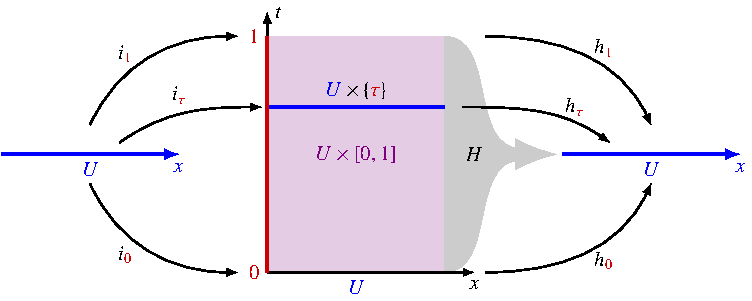
\includegraphics{chapters/060-pformen/images/homotopie.pdf}
\caption{Eine Homotopie $H$ ist eine Abbildung $U\times[0,1]$, die
die Abbildung $h_0\colon U\to U$ in die Abbildung $h_1\colon U\to U$
deformiert.
Die Abbildung $h_{\tau}$ entsteht durch Einsetzen des Wertes $\tau$
in das zweite Argument von $H$, was gleichbedeutend ist mit der
Zusammensetzung von $H$ mit $i_\tau$: $h_\tau=H\circ i_\tau$.
\label{buch:pformen:fig:homotopie}}
\end{figure}
%
Ist die 1-Form $\alpha$ auf einem offenen Ball $U\subset \mathbb{R}^n$
geschlossen, dann kann man eine Funktion $f$ finden, deren Differential
$df=\alpha$ ist.
Die Funktion $f$ entsteht durch Wegintegration z.~B.~vom Nullpunkt zum
Punkt $x$
\[
\gamma_x
\colon [0,1] \to U
:
t\mapsto \gamma_x(t) = xt.
\]
Betrachtet man $\gamma_x(t)$ als eine Funktion von zwei Variablen
$x$ und $t$, dann kann man sie schreiben als
\[
H
\colon
U\times[0,1]
\to
U
:
(x,t) \mapsto tx.
\]
Für jeden Wert von $t$ ist die partielle Funktion
\[
h_t \colon U \to U : x \mapsto tx
\]
eine Selbstabbildung von $U$.
Für $t=0$ wird jeder Punkt auf $0$ abgebildet, die Abbildung $h_0$ ist
die konstante Abbildung auf den Nullpunkt von $U$.
Für $t=1$ ist $h_1(x)=x$, $h_1$ ist also die identische Abbildung 
Man nennt $H$ eine {\em Homotopie} zwischen der konstanten Abbildung
und der identischen Abbildung.

Das Definitionsgebiet der Homotopie ist das karteische Produkt
$U\times[0,1]$.
Für jeden Wert von $\tau\in[0,1]$ ist die Abbildung
\[
i_\tau
\colon U \to U\times[0,1]
:
x\mapsto (x,\tau)
\]
eine Einbettung der $n$-dimensionalen Untermannigfaltigkeit $U$ in
$U\times[0,1]$.
Eine $(p+1)$-Form $\omega$ auf $U\times[0,1]$ wird durch $i_\tau^*$ zu
der $(p+1)$-Form $i_\tau^*(\omega)$, die durch
\begin{align*}
i_\tau^*\bigl(
f(x,t)
\,dx^{i_1}\wedge \dots \wedge dx^{i_p}\wedge dt
\bigr)
&=
0
\\
i_\tau^*\bigl(
g(x,t)
\,dx^{i_1}\wedge \dots \wedge dx^{i_p}\wedge dx^{i_{p+1}}
\bigr)
&=
g(x,\tau)
\,dx^{i_1}\wedge \dots \wedge dx^{i_p}\wedge dx^{i_{p+1}}
\end{align*}
sind, je nachdem ob die Form das Monom $dt$ enthält oder nicht.
Die Variable $t$ wird als Konstante mit dem Wert $\tau$ betrachtet.

%
% Faserintegration
%
\subsection{Faserintegration
\label{buch:pformen:poincare:subsection:faserintegration}}
%
% fig-faserintegration.tex
%
% (c) 2025 Prof Dr Andreas Müller
%
\begin{figure}
\centering
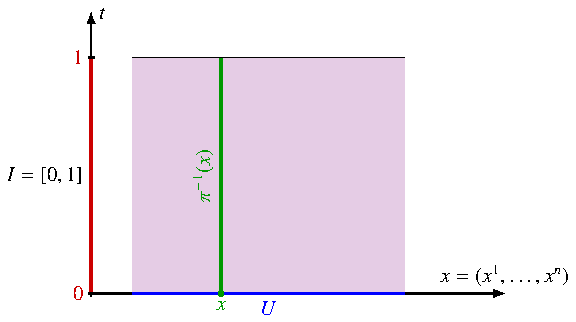
\includegraphics{chapters/060-pformen/images/faserintegration.pdf}
\caption{Die Projektion $\pi(x,t)=x$ projiziert die grünen Fasern
auf Punkte in $U$. Die Faserintegration integriert über solche Fasern
und reduziert damit den Grad einer $p+1$-Form auf $U\times [0,1]$
auf eine $p$-Form.
\label{buch:pformen:poincarelemma:fig:faserintegration}}
\end{figure}
%
Zu jeder $(p+1)$-Form $\omega$ mit $d\omega=0$ muss eine $p$-Form gefunden
werden.
Dazu müssen einzelne Faktoren $dx^i$ in einem Produkt
$dx^{i_1}\wedge\dots\wedge dx^{i_{p+1}}$ zum Verschwinden gebracht
werden.
Die einzige Möglichkeit, dies zu tun, ist über einzelne Koordinaten zu
integrieren.
Dies ist das Prinzip der Faser-Integration, die im folgenden Satz
definiert wird.

Für den Rest dieses Abschnitts verwenden wir folgende Notation.
Da es nur um lokale Fragen geht, können wir uns auf einzelne
Kartengebiete beschränken.
Wir betrachten daher Differentialformen auf einem offenen Ball
$U\subset\mathbb{R}^n$, in dem wir die Koordinaten mit $x^1,\dots,x^n$
bezeichnen.
Die Projektion $\pi$ ist die Abbildung
\[
\pi
\colon U \times [0,1]\to U : (x,t) \mapsto x,
\]
sie ist in Abbildung~\ref{buch:pformen:poincarelemma:fig:faserintegration}
dargestellt.

Die Projektion $\pi$ ermöglicht, eine $p$-Form $\omega$ auf $U$ in eine
$p$-Form $\pi^*(\omega)$ auf $U\times [0,1]$ abzubilden.
Wir benötigen aber eine andere Art von Abbildung.
Aus einer $(p+1)$-Form auf $U\times[0,1]$ möchten wir eine $p$-Form auf
$U$ erzeugen.
Dazu integrieren wir über die $t$-Koordinate, wie in der folgenden
Definition.

\begin{definition}
Die {\em Faserintegration} ist die linear Abbildung
\index{Faserintegration}%
$\pi_*\colon \Omega^{p+1}(U\times[0,1])\to\Omega^p(U)$,
die auf Basisformen durch
\begin{align*}
\alpha
&=
a_{i_1 \dots i_p}(x,t)
\,
dx^{i_1}\wedge\dots\wedge dx^{i_p}\wedge dt
&&\Rightarrow&
\pi_*\bigl(
\alpha
\bigr)
&=
\biggl(
\int_0^1 a_{i_1 \dots i_p}(x,t)\,dt
\biggr)
\,
dx^{i_1}\wedge\dots\wedge dx^{i_p}
\\
\beta
&=
b_{i_1 \dots i_{p+1}}(x,t)
\,
dx^{i_1}\wedge \dots \wedge dx^{i_{p+1}}
&&\Rightarrow&
\pi_*\bigl(\beta)
\bigr)
&=
0
\end{align*}
definiert ist.
\end{definition}

Die Faserintegration wirkt also nur auf $p$-Formen, die den Faktor $dt$
enthält.
Solche Faktoren werden über die Variable $t$ integriert.

Die Faserintegration ist nicht aus einer Abbildung der unterliegenden
Mannigfaltigkeiten entstanden (das wäre die Abbildung $\pi^*$).
Daher muss im nächsten Schritt ermittelt werden, wie Faserintegration
sich mit der äusseren Ableitung von Formen verträgt.

\begin{satz}[Faserintegration]
Sei $\omega\in\Omega^{p+1}(U\times[0,1])$ eine $(p+1)$-Form auf $U\times[0,1]$.
Dann  ist
\begin{equation}
\pi_*d\omega - d\pi_*\omega 
=
(-1)^{p+1}(i_1^*\omega- i_0^*\omega).
\label{buch:pformen:poincarelemma:eqn:pid}
\end{equation}
\end{satz}

\begin{proof}
Wir berechnen die Ableitungen und die Faserintegration der
Basis-$(p+1)$-Formen
\begin{align*}
\alpha
&=
a_{i_1 \dots i_p}(x,t)
\,
dx^{i_1}\wedge \dots \wedge dx^{i_p}\wedge dt
\\
\beta
&=
b_{i_1 \dots i_p i_{p+1}}(x,t)
\,
dx^{i_1}\wedge \dots \wedge dx^{i_p}\wedge dx^{i_{p+1}}
\end{align*}
auf $U\times[0,1]$.

Da $\alpha$ bereits $dt$ enthält, kommen in $d\alpha$ keine Ableitungen
von $a_{i_1\dots i_p}$ nach der Zeit vor.
Die Ableitungen sind:
\begin{align*}
d\alpha
&=
\sum_{k=1}^n \frac{\partial a_{i_1\dots i_p}(x,t)}{\partial x^k}
\,dx^k\wedge dx^{i_1}\wedge \dots \wedge dx^{i_p}\wedge dt
\qquad\qquad\text{und}
\\
d\beta
&=
\sum_{k=1}^n \frac{\partial b_{i_1\dots i_{p+1}}(x,t)}{\partial x^k}
\,dx^k\wedge dx^{i_1}\wedge \dots \wedge dx^{i_{p+1}}
+
\frac{\partial b_{i_1\dots i_{p+1}}(x,t)}{\partial t}
\,dt\wedge dx^{i_1}\wedge \dots\wedge dx^{i_{p+1}}.
\intertext{Die Faserintegration erhält nur die Terme mit $dt$ und 
ergibt}
\pi_*d\alpha
&=
\sum_{k=1}^n
\biggl(
\int_0^1 \frac{\partial a_{i_1\dots i_p}(x,t)}{\partial x^k}
\,dt
\biggr)
\,
dx^k
\wedge
dx^{i_1}\wedge\dots\wedge dx^{i_p}
\qquad\qquad\text{bzw.}
\\
\pi_*d\beta
&=
\biggl(
\int_0^1
\frac{\partial b_{i_1 \dots i_{p+1}}(x,t)}{\partial t}
\,dt
\biggr)
\,
(-1)^{p+1}
\,
dx^{i_1}\wedge\dots \wedge dx^{i_{p+1}}
\\
&=
\Bigl(
b_{i_1\dots i_{p+1}}(x,1)
-
b_{i_1\dots i_{p+1}}(x,0)
\Bigr)
\,
(-1)^{p+1}
\,
dx^{i_1}\wedge\dots\wedge dx^{i_p}\wedge dx^{i_{p+1}}.
\intertext{Die beiden Summanden im letzten Ausdruck entstehen dadurch,
dass die Variable $t$ auf $0$ bzw.~$1$, das ist}
&=
(-1)^{p+1}
\bigl(
i_1^*\beta - i_0^*\beta
\bigr).
\end{align*}

Wir berechnen jetzt die Wirkung der Operatoren $\pi^*$ und $d$ in der
umgekehrten Reihenfolge.
Da $\pi^*\beta=0$ ist auch $d\pi^*\beta=0$.
Für $\alpha$ ist etwa mehr Arbeit notwendig.
\begin{align*}
d\pi_*\alpha
&=
\sum_{k=1}^n
\frac{\partial}{\partial x_k}
\biggl(
\int_0^1 a_{i_1\dots i_p}(x,t)\,dt
\biggr)
dx^k\wedge dx^{i_1}\wedge\dots\wedge dx^{i_p}
\intertext{Die Ableitung kann ins Integral genommen werden und ergibt}
&=
\sum_{k=1}^n
\biggl(
\int_0^1 \frac{\partial a_{i_1\dots i_p}(x,t)}{\partial x_i} \,dt
\biggl)
\,
dx^k
\wedge
dx^{i_1}\wedge\dots\wedge dx^{i_p}
\\
&=
\pi_*d\alpha.
\end{align*}

Die Rechnung in den vorangegangenen Absätzen zeigt also, dass
\begin{align}
\pi_*d\alpha - d\pi_*\alpha
&=
0,
\label{buch:pformen:poincarelemma:eqn:i*alpha}
\\
\pi_*d\beta - d\pi_*\beta
&=
(-1)^{p+1}
\bigl(
i_1^*\beta - i_0^*\beta
\bigr).
\notag
\end{align}
Da in den Termen der Form $\alpha$ immer der Faktor $dt$ vorkommt, 
der von $i_\tau^*$ auf $0$ abgebildet wird, gilt $i_t^*\alpha=0$
und man kann die Null auf der rechten Seite von 
\eqref{buch:pformen:poincarelemma:eqn:i*alpha}
ebenfalls als
\(
\pi_*d\alpha-d\pi*\alpha=(-1)^{p+1}\bigl(i_1^*\alpha-i_0^*\alpha\bigr)
\)
schreiben.
Damit ist die Formel
\eqref{buch:pformen:poincarelemma:eqn:pid}
bewiesen.
\end{proof}

%
% Homotopie-Abbildung
%
\subsection{Homotopie-Abbildung
\label{buch:pformen:poincare:subsection:homotopie}}
Die Homotopie $H\colon U\times[0,1]\to U$ ist eine differenzierbare
Abbildung.
Die induzierte Abbildung $H^*\colon\Omega^*(U)\to\Omega^*(U\times[0,1])$
vertauscht mit $d$.
Für eine $p$-Form $\omega$ auf $U$ ist $H^*\omega$ eine $p$-Form auf
$U\times[0,1]$.
Entsprechend ist $\pi_*H^*\omega$ ist eine $(p-1)$-Form auf $U$.
Wir definieren daher die Funktion $J=\pi_*H^*$ und berechnen das
Verhalten mit der äusseren Ableitung.

\begin{satz}
\label{buch:pformen:poincarelemma:satz:homotopie}
Für jede $p$-Form $\omega\in\Omega^p(U)$ gilt
\[
Jd\omega - dJ\omega
=
(-1)^p(
h_1^*\omega - h_0^*\omega
)
\]
\end{satz}

\begin{proof}
\begin{align*}
J d \omega - d J \omega
&=
\pi_* H^* d \omega
-
d \pi^* H^* \omega
\\
&=
\pi_* d H^* \omega
-
d \pi^* H^* \omega
\\
&=
d \pi_* H^* \omega
+
(-1)^p(i_1^* H^* \omega - i_0^* H^* \omega)
-
d \pi^* H^* \omega.
\intertext{Der erste und der letzte Term heben sich weg.
Im mittleren Term ist $H\circ i_\tau=h_\tau$ und daher
$i_\tau^* H^* = (H\circ i_\tau)^* = h_\tau^*$.
Somit folgt}
J d \omega - d J \omega
&=
(-1)^p(h_1^* \omega - h_0^* \omega).
\end{align*}
wie behauptet.
\end{proof}

%
% Geschlossene Formen sind exakt
%
\subsection{Geschlossene Formen sind exakt
\label{buch:pformen:geschlossen:subsection:exakt}}
Mit der Faserintegration und der Homotopie-Abbildung wurde
in Abschnitt~\ref{buch:pformen:poincare:subsection:homotopie}
die Abbildung $J$ konstruiert, deren Eigenschaften im
Satz~\ref{buch:pformen:poincarelemma:satz:homotopie}
zusammengestellt wurden.
Damit ist es jetzt möglich, das Poincaré-Lemma zu beweisen.

\begin{satz}[Poincaré-Lemma]
\label{buch:pformen:geschlossen:satz:poincare-lemma}
Ist die $p$-Form $\omega\in\Omega^p(U)$ geschlossen, also $d\omega=0$,
dann gibt es eine $(p-1)$-Form $\alpha\in\Omega^{p-1}(U)$ mit
$d\alpha=\omega$.
\end{satz}

\begin{proof}
Nach Satz~\ref{buch:pformen:poincarelemma:satz:homotopie} folgt
wegen $d\omega=0$ sofort
\[
-dJ\omega
=
(-1)^p(h_1^*\omega - h_0^*\omega).
\]
Die Abbildung $h_0$ ist die konstante Abbildung $x\mapsto 0$, also ist ist
$h_0^*\omega=0$.
$h_1$ ist die identische Abbildung $x\mapsto x$, daher ist auch $h_1^*$
die identische Abbildung von $\Omega^*(U)$ und daher $h_1^*\omega=\omega$.
Damit folgt $dJ\omega=\omega$.
Somit ist $\alpha =(-1)^{p+1}J\omega$ die gesuchte $(p-1)$-Form.
\end{proof}

Wir prüfen nach, dass der ursprünglich für geschlossene 1-Formen
$\omega$ gegebene Beweis die gleiche Funktion
$f=J\omega\in\Omega^0(U)=C^\infty(U)$ mit $df=\omega$ ergibt.
Für eine 1-Form
\[
\omega = \sum_{i=1}^nf_i(x)\, dx^i
\]
ist zunächst
\[
H^*\omega
=
\sum_{i=1}^nf_i(tx)\, d(tx^i)
=
\sum_{i=1}^nf_i(tx) (x_i\, dt + t\, dx^i).
\]
Darauf muss jetzt die Operation $\pi_*$ angewendet werden.
Diese ergibt aber ein nicht verschwindendes Resultat nur auf Termen, in
denen $dt$ vorkommt.
Daher ist
\[
\pi_*H^*\omega
=
\int_0^1
\sum_{i=1}^n
f_i(tx) x^i\, dt
=
\int_0^1
\sum_{i=1}^n
f_i(\gamma_x(t)) \dot{x}^i(t)\, dt
=
\int_{\gamma_x}
\omega.
\]
Die von der Abbildung $J$ produzierte Funktion ist also im Falle
einer 1-Form gerade das Wegintegral über einen Weg vom Nullpunkt zum
Punkt $x$, wie in der ursprünglichen Konstruktion in
Kapitel~\ref{chapter:kurvenintegral}.





